\section{Classification of Living Things} \index{Classification}

\begin{multicols}{2}


\section*{Concept of Classification}


\subsection{Arranging Shapes} % Source 26

\begin{center}
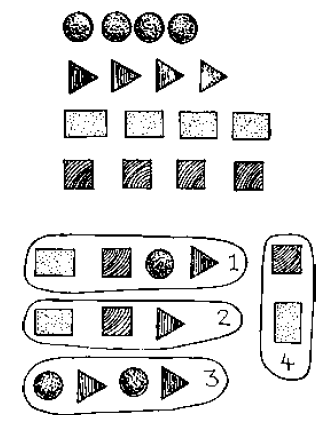
\includegraphics[width=0.4\textwidth]{./img/source/arranging-shapes.png}
\end{center}

\begin{description*}
%\item[Subtopic:]{}
\item[Materials:]{Paper/card, coloured pens/pencils}
%\item[Setup:]{}
\item[Procedure:]{Make four of each of the following shapes: squares (3 cm $\times$ 3 cm) triangle (3 cm sides)
rectangles (3 $\times$ 4 cm) circles (3 cm diameter). Mix the shapes and then sort them according to
a chosen feature.}
%\item[Hazards:]{}
\item[Questions:]{How many different ways can you find of grouping the shapes?}
\item[Observations:]{At least 4 can be found.}
\item[Theory:]{In Biology, classification is used to group things based on shared qualities (i.e. living and non-living things).}
%\item[Applications:]{}
%\item[Notes:]{}
\end{description*}

\vfill
\columnbreak

\subsection{Classification at the Duka} % Source 27

\begin{center}
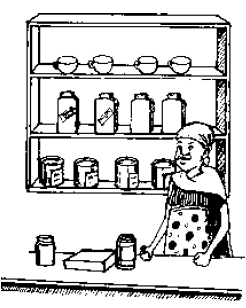
\includegraphics[width=0.38\textwidth]{./img/source/classification-duka.png}
\end{center}

\begin{description*}
%\item[Subtopic:]{}
%\item[Materials:]{}
%\item[Setup:]{}
\item[Procedure:]{Observe how goods at the local shop are arranged on the shelves.}
%\item[Hazards:]{}
\item[Questions:]{Can you find a pattern in the arrangements on the shelves?}
\item[Observations:]{The goods will be arranged firstly in large groups, i.e. foodstuffs, non-food stuffs (medicines,
etc.), and then into smaller groups such as foods in tins, foods in bottles, etc.}
\item[Theory:]{This concept of classification is also used in the study of Biology.}
%\item[Applications:]{}
%\item[Notes:]{}
\end{description*}

\subsection{Find a Missing Person}

\begin{center}
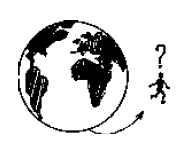
\includegraphics[width=0.35\textwidth]{./img/source/missing-person.png}
\end{center}

\begin{description*}
%\item[Subtopic:]{}
%\item[Materials:]{}
%\item[Setup:]{}
\item[Procedure:]{Imagine that you have been asked to find one particular person on earth.}
%\item[Hazards:]{}
\item[Questions:]{What information would you require?}
\item[Observations:]{Continent, country, region, district, ten cell block, house, name of person.}
\item[Theory:]{This procedure can be compared to the process of classifying organisms, firstly in large
groups (equivalent to a continent), then smaller groups (equivalent to country, region etc).}
%\item[Applications:]{}
%\item[Notes:]{}
\end{description*}

\subsection{Classifying Leaves} % Source 28

\begin{center}
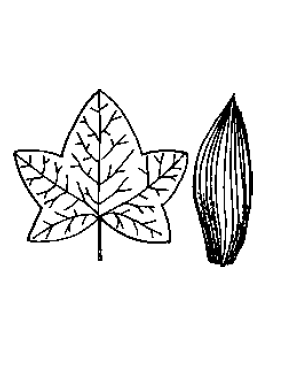
\includegraphics[width=0.4\textwidth]{./img/source/classify-leaves.png}
\end{center}

\begin{description*}
%\item[Subtopic:]{}
%\item[Materials:]{Various leaves}
%\item[Setup:]{}
\item[Procedure:]{Collect leaves from different plants. Make large groups and small groups using as many
different characteristics as possible.}
%\item[Hazards:]{}
\item[Questions:]{How many ways can you find to group the leaves?}
\item[Observations:]{Characteristics like shape, colour, vein pattern, leaf margin etc. can all be used.}
%\item[Theory:]{}
%\item[Applications:]{}
%\item[Notes:]{}
\end{description*}

\subsection{Scavenger Hunt} % Shika 223

%\begin{center}
%\includegraphics[width=0.4\textwidth]{./img/.png}
%\end{center}

\begin{description*}
%\item[Subtopic:]{}
%\item[Materials:]{}
%\item[Setup:]{}
\item[Procedure:]{Find different animals, plants, fungi etc. that are available around the school or at their homes (especially mosses in wet places and fungi near decaying material in the shade). Send students to find different specimen giving hints if necessary. When they return, have them classify what has been found.}
%\item[Hazards:]{}
%\item[Questions:]{}
%\item[Observations:]{}
%\item[Theory:]{}
%\item[Applications:]{}
%\item[Notes:]{}
\end{description*}

\vfill
\columnbreak

\subsection{Display Boards} \index{Displays} \index{Visual aids} % VSO 19, Source

\begin{center}
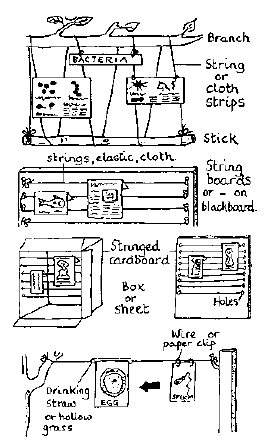
\includegraphics[width=0.49\textwidth]{./img/source/displays.png}
\end{center}

\begin{description*}
%\item[Subtopic:]{}
\item[Materials:]{String, sticks/branches, cardboard boxes, nails, tape}
%\item[Setup:]{}
\item[Procedure:]{Construct display boards as shown to present information about specimen collected. Students can present their displays to the class or as part of a science fair project.}
%\item[Hazards:]{}
%\item[Questions:]{}
%\item[Observations:]{}
%\item[Theory:]{}
%\item[Applications:]{}
\item[Notes:]{See more display ideas in \nameref{cha:displays} (p.~\pageref{cha:displays}).}
\end{description*}

%==================================================================================================%


\end{multicols}

\pagebreak